\documentclass{article}
\usepackage{graphicx}
\usepackage{geometry}
\usepackage{listings}

\geometry{
	a4paper,
	total={210mm,297mm},
	left=20mm,
	right=20mm,
	top=20mm,
	bottom=20mm,
}
\begin{document}
	
	\begin{center}
		\textbf{\bfseries\Large ASSIGNMENT NO. 8}
		\\[1cm]
	\end{center}
	\section{TITLE : } Implementation of K-NN approach take suitable example.
	\section{OBJECTIVE : }  To understand the working of KNN Algorithm.
	\section{SOFTWARE REQUIREMENTS : }
	\begin{itemize}
		\item Linux Operating System
		\item Python Compiler
	\end{itemize}
	
	\section{THEORY : }
	\subsection{What is k-Nearest Neighbors :}
	The model for kNN is the entire training dataset. When a prediction is re-
	quired for a unseen data instance, the kNN algorithm will search through the
	training dataset for the k-most similar instances. The prediction attribute
	of the most similar instances is summarized and returned as the prediction
	for the unseen instance.
	The similarity measure is dependent on the type of data. For real-valued
	data, the Euclidean distance can be used. Other other types of data such as
	categorical or binary data, Hamming distance can be used.
	In the case of regression problems, the average of the predicted attribute
	may be returned. In the case of classication, the most prevalent class may
	be returned. 
	\subsection{How does k-Nearest Neighbors Work :}
	The kNN algorithm is belongs to the family of instance-based, competitive
	learning and lazy learning algorithms.
	Instance-based algorithms are those algorithms that model the problem us-
	ing data instances (or rows) in order to make predictive decisions. The kNN algorithm is an extreme form of instancebased methods because all training
	observations are retained as part of the model.
	It is a competitive learning algorithm, because it internally uses competi-
	tion between model elements (data instances) in order to make a predictive
	decision. The objective similarity measure between data instances causes
	each data instance to compete to win or be most similar to a given unseen
	data instance and contribute to a prediction.
	Lazy learning refers to the fact that the algorithm does not build a model
	until the time that a prediction is required. It is lazy because it only does
	work at the last second. This has the beneft of only including data relevant
	to the unseen data, called a localized model. A disadvantage is that it can be
	computationally expensive to repeat the same or similar searches over larger
	training datasets.Finally, kNN is powerful because it does not assume anything about the
	data, other than a distance measure can be calculated consistently between
	any two instances. As such, it is called nonparametric or non-linear as it
	does not assume a functional form.
	
	\subsection{Classify Flowers Using Measurements :}
	This Program is broken down into the following steps:\\
	\newpage
	\begin{figure}[h!]
		\centering
		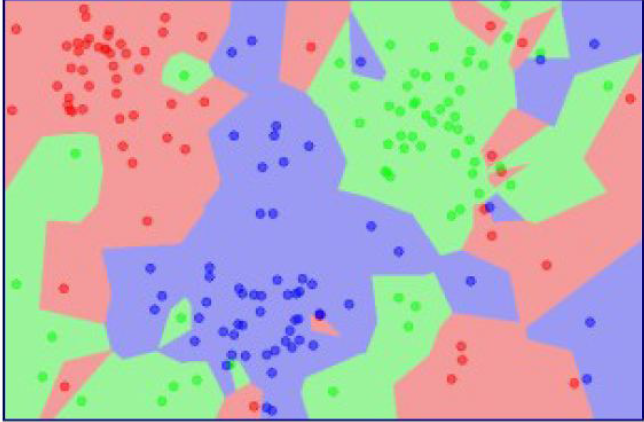
\includegraphics[scale=0.5]{204/Assignment No -8(KNN )daa/knnkifig.png}
	\end{figure}
	\begin{enumerate}
		\item \textbf{Handle Data} : Open the dataset from CSV and split into test/train datasets.
		\item \textbf{Similarity}  : Calculate the distance between two data instances.
		\item \textbf{Neighbors}   : Locate k most similar data instances.
		\item \textbf{Response}    : Generate a response from a set of data instances.
		\item \textbf{Accuracy}    : Summarize the accuracy of predictions.
		\item \textbf{Main}        : Tie it all together.
	\end{enumerate}
	\begin{enumerate}
		\item \textbf{Handle Data :}\\The first thing we need to do is load our data file. The data is in CSV format without a header line or any quotes. We can open thefle with the open function and read the data lines using the reader function in the csv module.\\import csv with open(`iris.data', `rb') as csvfle: lines =csv.reader(csvfle)for row in lines: print ', `.join(row)\\Next we need to split the data into a training dataset that kNN can use to make predictions and a test dataset that we can use to evaluate
		the accuracy of the model.\\We first need to convert the ower measures that were loaded as strings
		into numbers that we can work with. Next we need to split the data set randomly into train and datasets. A ratio of 67/33 for train/test is a standard ratio used.\\Pulling it all together, we can define a function called loadDataset that loads a CSV with the provided lename and splits it randomly into train and test datasets using the provided split ratio.\\import csv
		import random
		def loadDataset(lename, split, trainingSet=[] , testSet=[]): with
		open(lename, 'rb') as csvle: lines = csv.reader(csvle) dataset =
		list(lines) for x in range(len(dataset)-1): for y in range(4): dataset[x][y]
		= 
		oat(dataset[x][y])
		if random.random() < split: trainingSet.append(dataset[x]) else: test-
		Set.append(dataset[x])
		Download the iris 
		owers dataset CSV le to the local directory. We
		can test this function out with our iris dataset, as follows:
		trainingSet=[] testSet=[] loadDataset(`iris.data', 0.66, trainingSet, test-
		Set) print `Train: ' + repr(len(trainingSet)) print `Test: ' + repr(len(testSet))
		\item \textbf{Similarity :}\\In order to make predictions we need to calculate the similarity be-
		tween any two given data instances. This is needed so that we can locate the k most similar data instances in the training dataset for a given member of the test dataset and in turn make a prediction. Given that all four  ower measurements are numeric and have the same
		units, we can directly use the Euclidean distance measure. This is defined as the square root of the sum of the squared diferences between the two arrays of numbers (read that again a few times and let it sink
		Additionally, we want to control which fields to include in the distance calculation. Specically, we only want to include the first 4 attributes.
		One approach is to limit the euclidean distance to a xed length, ig-noring the final dimension.
		Putting all of this together we can define the euclidean Distance\\
		function as follows:\\
		import math\\
		def euclideanDistance(instance1, instance2, length): distance = 0 for
		x in range(length): distance += pow((instance1[x] - instance2[x]), 2)
		return math.sqrt(distance)
		\item \textbf{Neighbors :}
		Now that we have a similarity measure, we can use it collect the k
		most similar instances for a given unseen instance.
		This is a straight forward process of calculating the distance for all
		instances and selecting a subset with the smallest distance values.
		Below is the getNeighbors function that returns k most similar neigh-
		bors from the training set for a given test instance (using the already
		defined euclidean Distance function)\\import operator\\
		def getNeighbors(trainingSet, testInstance, k): distances = [] length =
		len(testInstance)-1
		for x in range(len(trainingSet)): dist = euclideanDistance(testInstance,
		trainingSet[x], length) distances.append((trainingSet[x], dist))
		distances.sort(key=operator.itemgetter(1)) neighbors = []
		for x in range(k): neighbors.append(distances[x][0])
		return neighbors\\We can test out this function as follows:\\trainSet = [[2, 2, 2, `a'], [4, 4, 4, `b']] testInstance = [5, 5, 5] k =
		1
		neighbors = getNeighbors(trainSet, testInstance, 1) print(neighbors)
		\item \textbf{Response :}
		Once we have located the most similar neighbors for a test instance,
		the next task is to devise a predicted response based on those neighbors.
		We can do this by allowing each neighbor to vote for their class at-
		tribute, and take the majority vote as the prediction.
		Below provides a function for getting the majority voted response from
		a number of neighbors. It assumes the class is the last attribute for
		each neighbor.\\import operator
		def getResponse(neighbors): classVotes = fg
		for x in range(len(neighbors)): response = neighbors[x][-1] if response
		in classVotes: classVotes[response] += 1
		else: classVotes[response] = 1 sortedVotes = sorted(classVotes.iteritems(),
		key=operator.itemgetter(1), reverse=True) return sortedVotes[0][0]\\We can test out this function with some test neighbors, as follows:\\neighbors = [[1,1,1,`a'], [2,2,2,`a'], [3,3,3,`b']] response = getResponse(neighbors)
		print(response)\\This approach returns one response in the case of a draw, but you
		could handle such cases in a specic way, such as returning no response
		or selecting an unbiased random response.
		\item \textbf{Accuracy :}
		We have all of the pieces of the kNN algorithm in place. An important
		remaining concern is how to evaluate the accuracy of predictions.
		An easy way to evaluate the accuracy of the model is to calculate a
		ratio of the total correct predictions out of all predictions made, called
		the classication accuracy.
		Below is the getAccuracy function that sums the total correct predic-
		tions and returns the accuracy as a percentage of correct classications.
		def getAccuracy(testSet, predictions): correct = 0\\for x in range(len(testSet)): if testSet[x][-1] is predictions[x]: correct
		+= 1
		return (correct/
		oat(len(testSet))) * 100.0
		We can test this function with a test dataset and predictions, as follows:
		testSet = [[1,1,1,`a'], [2,2,2,`a'], [3,3,3,`b']] predictions = [`a', `a', `a']
		accuracy = getAccuracy(testSet, predictions) print(accuracy)
		\item \textbf{Main :}We now have all the elements of the algorithm and we can tie them
		together with a main function.
		
	\end{enumerate}
	\section{MATHMATICAL MODEL :}
	Consider a set S consisting of all the elements related to a program.The
	mathematical model is given as below,
	S=fs,e,X,Y,Fme,DD,NDD,Mem sharedg\\Where,\\
	s = Initial State\\
	e = End State\\
	X = Input. Here it is iris dataset (in CSV format).\\
	Y = Output.Here output is accuracy of predictions related to the iris dataset.\\
	Fme = Algorithm/Function used in program. for eg.floadDataset(),euclidianDistance(),
	getNeighbors(),getResponse(),getAccuracy()g\\
	DD=Deterministic Data\\
	NDD=Non deterministic Data\\
	Mem shared=Memory shared by processor.
	\section{CONCLUSION :}
	Thus, we have implemented KNN approach for the iris dataset.
	\begin{center}
		\begin{tabular}{|c|c|c|c|c|}
			\hline	
			•Roll No &  Name of Student & Date of Performance & Date of Checking &  Signature of Staff\\ \hline
			•BECOC357      & Sunny Shahr     & 05 / 10 / 2017                                  & 05 / 10 / 2017                             &  \\ \hline
		\end{tabular}•
	\end{center}
	
	
	\section{PLAGARISM REPORT :}
	\begin{figure}[h!]
		\centering
		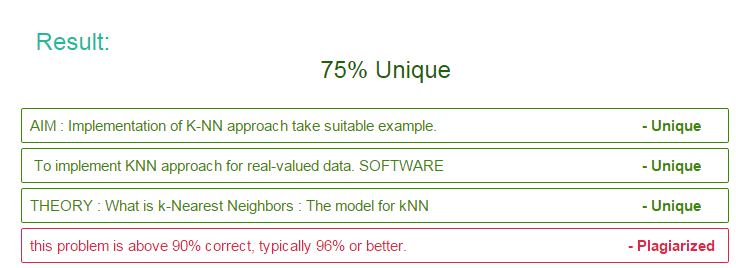
\includegraphics{204/Assignment No -8(KNN )daa/knnorig.png}
		\caption{Plagarism Checker: www.smallseotools.com/plagarism-checker}
	\end{figure}
\end{document}